 
% Appendix B

\chapter{Demonstration System Architecture} % Main appendix title

\label{chapter:AppendixB} % For referencing this appendix elsewhere, use \ref{AppendixA}

Although the work presented does not promise a system that implements proposed mechanism, it is necessary to have a prototype to demonstrate the correct operation of anomaly detector, so this annex focuses on presenting both the physical and logical architecture of prototype.
%Si bien el trabajo presentado no promete un sistema que implemente el mecanisno propuesto, es necesario tener un prototipo para demostrar el correcto funcionamiento del detector de anomal\'{i}as, por lo que este anexo se centra en presentar la arquitectura tanto f\'{i}sica como l\'{o}gica del prototipo.

\section{Physical Architecture}

\begin{figure}[h!]
  \begin{center}	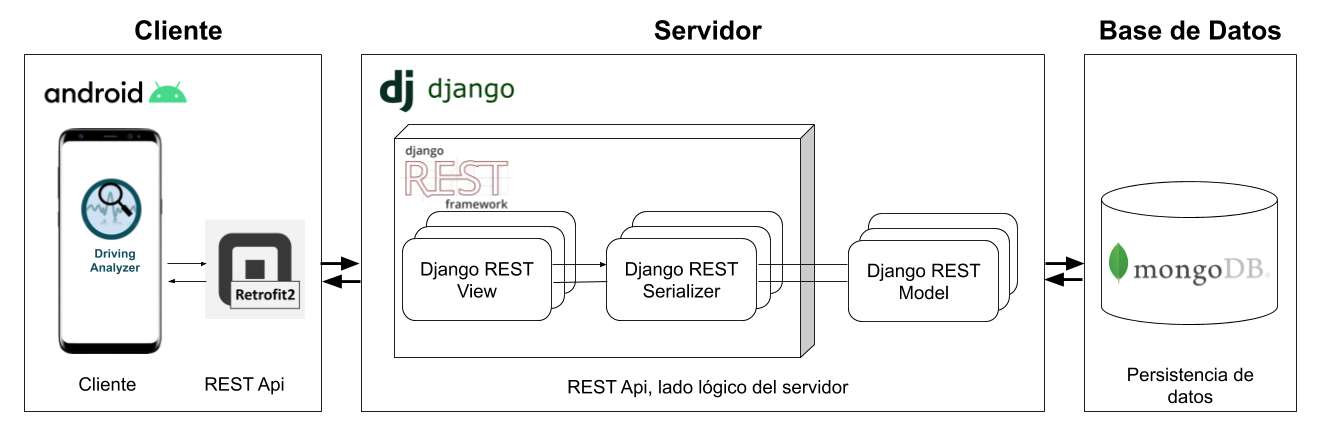
\includegraphics[width=0.95\textwidth, fbox]{imagenes/Apendices/Arquitectura}
  \caption{Physical architecture of Demonstration System (Own Elaboration).}
  \label{fig:arq_fis}  
  \end{center}
\end{figure}

Physical architecture of prototype has three main parts: client, server and database, as can be seen in Figure B.1. First of all client is made up of a mobile application for Android in charge of capturing data from inertial sensors, to later send them to server using Retrofit 2, later data enters the server made in Django, once server receives this data, it is in charge of preprocessing them to subsequently predict whether data sent is anomalous or not, and finally received data is stored in MongoDB Database with its respective prediction in order to monitor the user's driving.
%La arquitectura f\'{i}sica del prototipo cuenta con tres partes principales: el cliente, el servidor y la base de datos, como se puede observar en la Figura \ref{fig:arq_fis}. En primer lugar el cliente esta compuesto por una aplicaci\'{o}n m\'{o}vil para Android encargada de capturar los datos de los sensores inerciales, para posteriormente enviarlas al servidor usando Retrofit 2, posteriormente los datos ingresan al servidor realizado en Django, una vez el servidor recibe estos datos, se encarga de preprocesarlos para posteriormente predecir s\'{i} los datos enviados son anomal\'{i}as o no lo son, y por \'{u}ltimo los datos recibidos son almacenados en la Base de Datos de MongoDB con su respectiva predicci\'{o}n con el objetivo de hacer un monitoreo de la conducci\'{o}n del usuario.

\section{Logical Architecture} 

\begin{figure}[h!]
  \begin{center}	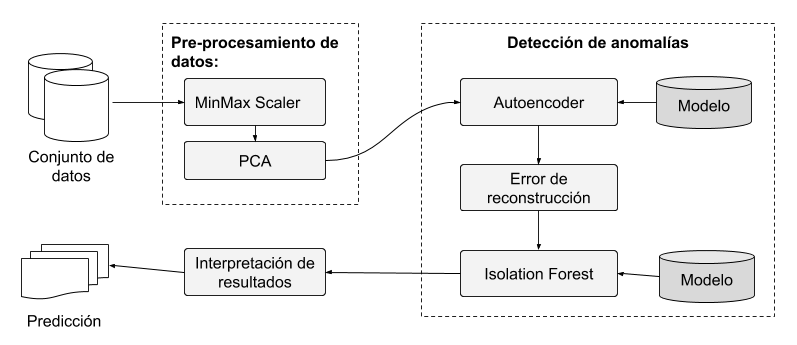
\includegraphics[width=0.95\textwidth, fbox]{imagenes/Apendices/arquitectura_logica}
  \caption{Logical Architecture of Demonstration System (Own elaboration).}
  \label{fig:arq_log}  
  \end{center}
\end{figure}

Regarding logical architecture, two main parts of the proposed detection mechanism are observed: pre-processing and anomaly detection, as can be seen in Figure \ref{fig:arq_log}.
%En cuanto a la arquitectura l\'{o}gica se observa las dos principales partes del mecanismo de detecci\'{o}n propuesto: el pre-procesamiento y la detecci\'{o}n de anomal\'{i}as, como se puede observar en la Figura \ref{fig:arq_log}.